\renewcommand{\theequation}{\theenumi}
\begin{enumerate}[label=\arabic*.,ref=\thesubsection.\theenumi]
\numberwithin{equation}{enumi}

\item let assume that the vertices of the rhombus are$\vec P$, $\vec Q$,$\vec R$ and $\vec S$ respectively as shown in fig(2.2.1).
finding out the $\vec{ SP}$ and $\vec {QP}$...
\begin{align}
	\vec {P} - \vec{S} &= \myvec{3 +2\\0+1}
	\\ &= \myvec{5\\1}
	\\
    \vec {Q} - \vec {P} &= \myvec{4-3\\5-0}
	\\ &= \myvec{1\\5}
\end{align}

\begin{figure}[!ht]
	\centering
	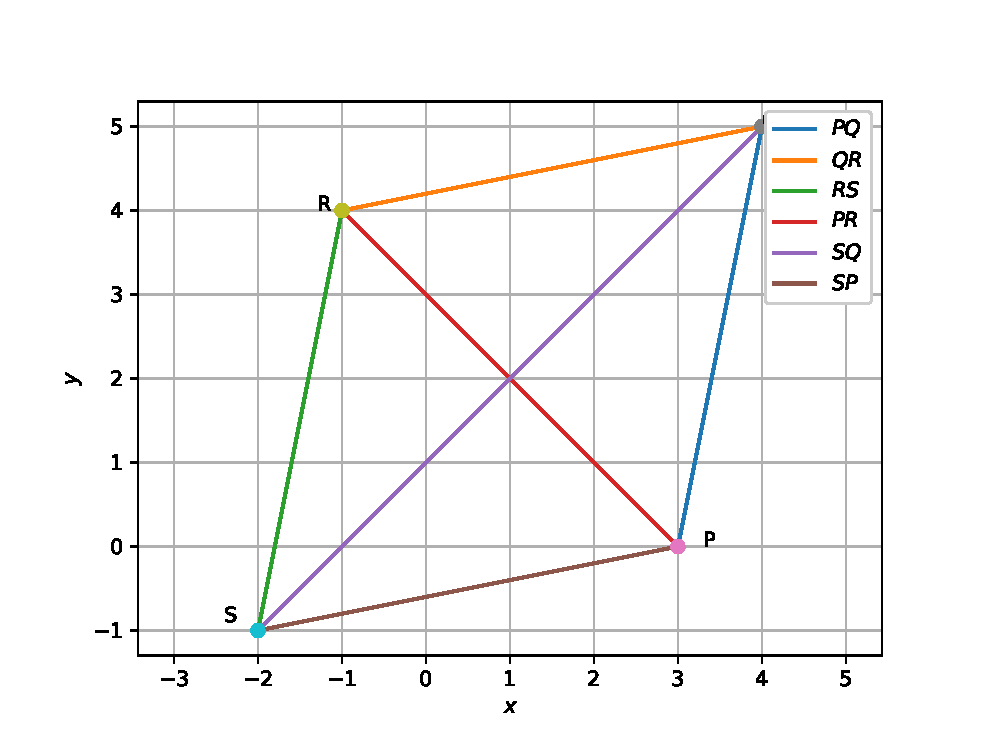
\includegraphics[width=\columnwidth]{./figures/quadrilateral/quad.eps}
	\caption{quadrilateral }
	\label{fig:quadrilateral}
	Path to the python code for the above figure
	\begin{lstlisting}
	codes/quadrilateral/quad.py
	\end{lstlisting}
\end{figure}


$\vec {S}$ Area of the rhombus can be calculated as follows 
\\
\begin{align}
	\norm{\Delta} &=\norm{ \mathbf{\left(\vec {P} - \vec {S}\right)} \times \mathbf{\left(\vec {Q} - \vec {P}\right)}}
	\\
	\norm{\Delta} &= \norm{ \mathbf{\myvec{5\\1}} \times \mathbf{\myvec{1\\5}}}
	\\
	\norm{\Delta} &= 5 \times 5 - 1 \times 1
	\\
	\norm{\Delta} &= 24
\end{align}

\end{enumerate}